% Latex template: mahmoud.s.fahmy@students.kasralainy.edu.eg
% For more details: https://www.sharelatex.com/learn/Beamer

\documentclass{beamer}					% Document class

\setbeamertemplate{footline}[text line]{%
  \parbox{\linewidth}{\vspace*{-8pt}Correlated dynamics in spiking neural networks\hfill\insertshortauthor\hfill\insertpagenumber}}
\setbeamertemplate{navigation symbols}{}

\usepackage[english]{babel}				% Set language
\usepackage[utf8x]{inputenc}			% Set encoding

\mode<presentation>						% Set options
{
  \usetheme{default}					% Set theme
  \usecolortheme{default} 				% Set colors
  \usefonttheme{default}  				% Set font theme
  \setbeamertemplate{caption}[numbered]	% Set caption to be numbered
}

% Uncomment this to have the outline at the beginning of each section highlighted.
%\AtBeginSection[]
%{
%  \begin{frame}{Outline}
%    \tableofcontents[currentsection]
%  \end{frame}
%}

\usepackage{graphicx}					% For including figures
\usepackage{booktabs}					% For table rules
\usepackage{hyperref}					% For cross-referencing

\title{Correlated dynamics in spiking neural networks}	% Presentation title
\author{Clayton W. Seitz}								% Presentation author
\date{\today}									% Today's date	

\begin{document}

% Title page
% This page includes the informations defined earlier including title, author/s, affiliation/s and the date
\begin{frame}
  \titlepage
\end{frame}

% Outline
% This page includes the outline (Table of content) of the presentation. All sections and subsections will appear in the outline by default.
\begin{frame}{Outline}
  \tableofcontents
\end{frame}

% The following is the most frequently used slide types in beamer
% The slide structure is as follows:
%
%\begin{frame}{<slide-title>}
%	<content>
%\end{frame}


\begin{frame}{Integrate and fire (IF) neuron models}

\begin{figure}
\centering
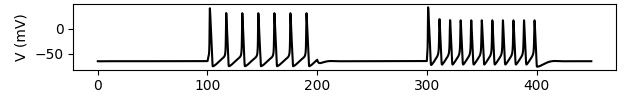
\includegraphics[width=100mm]{figure-19-1}
\end{figure}

\begin{figure}
\centering
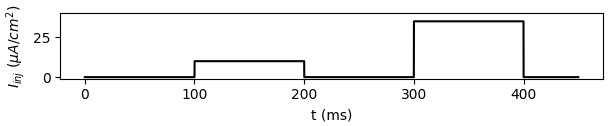
\includegraphics[width=100mm]{figure-19-2}
\end{figure}

\begin{equation*}
\tau\dot{V}(t) = g_{\ell}(E - V) + g_{\ell}\cdot \psi(V) + I(t)
\end{equation*}


\end{frame}

\begin{frame}{Monte-Carlo simulation of uncoupled IF neurons}

When $\psi(V) = g_{\ell}\Delta_{T}\exp\left(\frac{V-V_{L}}{\Delta_{T}}\right)$ we have the exponential integrate and fire model

\begin{figure}
\centering
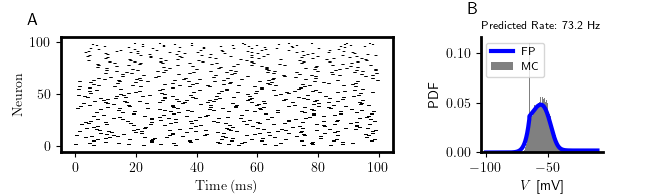
\includegraphics[width=100mm]{figure-3-1}
\end{figure}

Langevin equations have a corresponding Fokker-Planck equation 

\begin{equation*}
\frac{\partial P}{\partial t} = \frac{\sigma^{2}}{\tau}\frac{\partial^{2}P}{\partial V^{2}} + \frac{\partial}{\partial V}\left(\frac{V-E+\psi}{\tau}P\right)
\end{equation*}

\end{frame}


\begin{frame}{Synaptic coupling can induce correlations in spiking activity}

For special synaptic connectivity regimes dynamical variables can remain uncorrelated between neurons

\begin{figure}
\centering
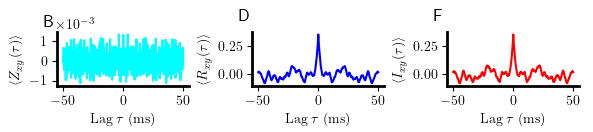
\includegraphics[width=100mm]{figure-12-1}
\end{figure}

Uncorrelated neural activity captures irregular spiking seen \emph{in-vivo}

\end{frame}

\section{Synaptic connectivity as an internal model}
\begin{frame}{Predicting neuron correlations}
The linear response of $r(t)$ allows us to also estimate the matrix of cross-correlations $C_{kj}(\tau)$
from the synaptic connectivity $\mathcal{C}$
\begin{figure}
\centering
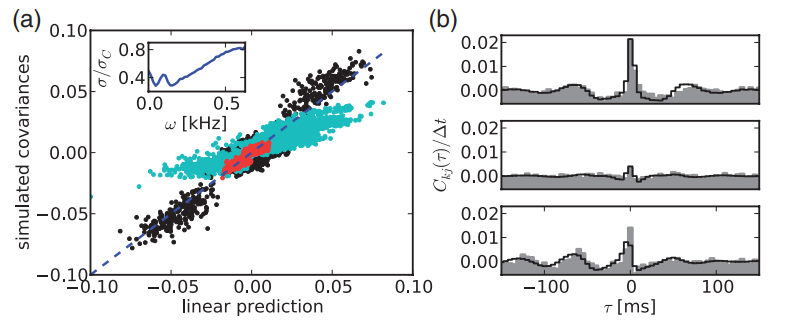
\includegraphics[width=110mm]{figure-20}
\end{figure}

This has important implications for brain-inspired machine learning

\end{frame}


\section{References}

% Adding the option 'allowframebreaks' allows the contents of the slide to be expanded in more than one slide.
\begin{frame}[allowframebreaks]{References}
	\tiny\bibliography{references}
	\bibliographystyle{apalike}
\end{frame}

\end{document}